\documentclass[letterpaper, 12pt]{report}

% insert any packages, environments, counters, etc here
\usepackage{graphicx}
\usepackage{hyperref}

\begin{document}
%insert document contents here

\chapter{Sequence Modeling: Recurrent and Recursive Nets}

\textbf{Recurrent Neural Networks} or RNNs are a family of neural networks for processing sequential data. 

\href{https://www.iro.umontreal.ca/~vincentp/ift3395/lectures/backprop_old.pdf}{Rumelhart et al, 1986a | Learning Representations by Back Propagating Errors}

\begin{quote}
  We describe a new learning procedure, back-propagation, for networks
  of neurone-like units. The procedure repeatedly adjusts the weights
  of the connections in the network so as to minimize a measure of the
  difference between the actual output vector of the net and the
  desired output vector. As a result of the weight adjustments,
  internal 'hidden' units which are not part of the input or output
  come to represent important features of the task domain, and the
  regularities in the task are captured by the interactions of these
  units. The ability to create useful new features distinguishes
  back-propagation from earlier, simpler methods such as the
  perceptron-convergence procedure.
\end{quote}

A RNN is a network that is specialized for processing a sequence of values $x^{(1)}, ..., x^{(\tau)}$. RNNs can scale to much longer sequences than would be practical for networks without sequence based specialization, and they can also process sequences of variable length. 

To go from multilayer networks to recurrent networks, we need to take advantage of parameter sharing. This makes it possible to extend and apply the model to examples of different forms and generalize across them. Such sharing is important when a specific piece of information can occur at multiple positions within the sequence.

A related idea is the use of convolution across a 1D temporal space. This approach is the basis for time delay neural networks. The convolution operation allows a network to share parameters across time, but it is shallow. The output of convolution is a sequence where each member of the output is a function of a small number of neighboring members of the input. The idea of parameter sharing in this case manifests in the application of the same convolution kernel at each time step.

Recurrent networks share parameters in a different way. Each member of the output is a function of the previous members of the output. Each output member is produced using the same update rule applied to the previous outputs. This formulation results in the sharing of parameters through a very deep computational graph. 

This chapter extends the idea of a computational graph to include cycles which represent the influence of the present value of a variable on its own value at a future time step. 

For more information on recurrent neural networks than is available in this chapter, look into \href{https://www.cs.toronto.edu/~graves/preprint.pdf}{Alex Graves | Supervised Sequence Labelling with Recurrent Neural Networks}

\section{Unfolding Computational Graphs}

In this section we explain the idea of \textbf{unfolding} a recursive or recurrent computation into a computational graph that has a repetitive structure, typically corresponding to a chain of events. Unfolding this graph results in the sharing of parameters across a deep network structure. 

Consider the classical form of a dynamical system: 

\begin{center}
  $s^{(t)} = f(s^{(t-1)}; \theta)$
\end{center}

where $s^{(t)}$ is the state of the system. This is recurrent because the definition of $s$ at time $t$ refers back to the same definition at time $t-1$. 

For a finite number of steps, we can unfold the graph by applying the definition $\tau - 1$ times. For example, if we unfold above 3 times:

\begin{center}
  $s^{(3)} = f(s^{(2)}; \theta) = f(f(s^{(1)}; \theta) \theta)$
\end{center}

By unfolding this repeatedly, we yield an expression that does not involve recurrence. Such an expression can now be represented by a traditional directed acyclic computational graph. 

\begin{figure}[h]
  \centering
  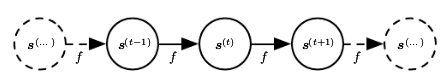
\includegraphics[width=0.7\textwidth]{trad_dag.png}
\end{figure}

Many recurrent networks also define their hidden units using recursive functions, such as 

\begin{center}
  $h^{(t)} = f(h^{(t-1)}, x^{(t)}; \theta)$
\end{center}

Typical RNNs will add extra architectural features such as output layers that read information out of the state $h$ to make predictions. When the network is trained to perform a task that requires predicting the future from the past, the network typically learns to use $h^{(t)}$ as a kind of lossy summary of the task relevant aspects of the past sequence of inputs up to $t$. This summary is in general necessarily lossy since it maps an arbitrary length sequence $(x^{(t)}, x^{(t-1)}, ..., x^{(2)}, x^{(1)})$ to a fixed length vector $h^{(t)}$. 

For example, if we were to use an RNN to predict the next word given the previous words, it may not be necessary to store all of the information in the input sequence up to time t, but instead only enough information to predict the rest of the sentence. The most demanding situation is when we ask $h^{(t)}$ to be rich enough to allow one to approximately recover the input sequence, as in autoencoder frameworks. 

\begin{figure}[h]
  \centering
  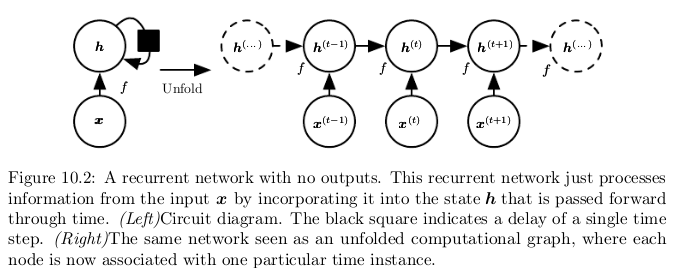
\includegraphics[width=0.7\textwidth]{rnn_dag.png}
\end{figure}

What we call unfolding is the operation that maps a circuit (as in the left side of above) to a computational graph with repeated pieces (as in the right side). The unfolded graph now has a size that depends on the sequence length. 

The unfolding process has two major advantages:

1. Regardless of the sequence length, the learned model always has the same input size, because it is specified in terms of transition from one state to another state, rather than specified in terms of a variable length history of states.

2. It is possible to use the same transition function $f$ with the same parameters at each step

2 follows because we can represent the unfolded recurrence after $t$ steps with a function $g$: 

\begin{center}
  $h^{(t)} = g^{(t)}(x^{(t)}, x^{(t-1)}, ..., x^{(2)}, x^{(1)}) = f(h^{(t-1)}x^{(t)}; \theta)$
\end{center}

The function $g^{(t)}$ takes the whole past sequence as input and produces the current state, but the unfolded recurrent structure allows us to factorize $g^{(t)}$ into repeated applications of a function $f$. 

The two advantages above allow us to learn a single model $f$ that operates on all time steps and all sequence lengths, rather than needing to learn a separate model $g^{(t)}$ for all possible time steps. Learning a single, shared model allows generalization to sequence lengths that did not appear in the training set and allows the model tobe estimated with far fewer training examples than would be required without parameter sharing. 

\section{Recurrent Networks}

Now that we know of graph unrolling and parameter sharing, we can design a wide variety of networks. Some examples of design patterns for RNNs include the following:

- RNNs that produce an output at each time step and have recurrent connections between hidden units

\begin{figure}[h]
  \centering
  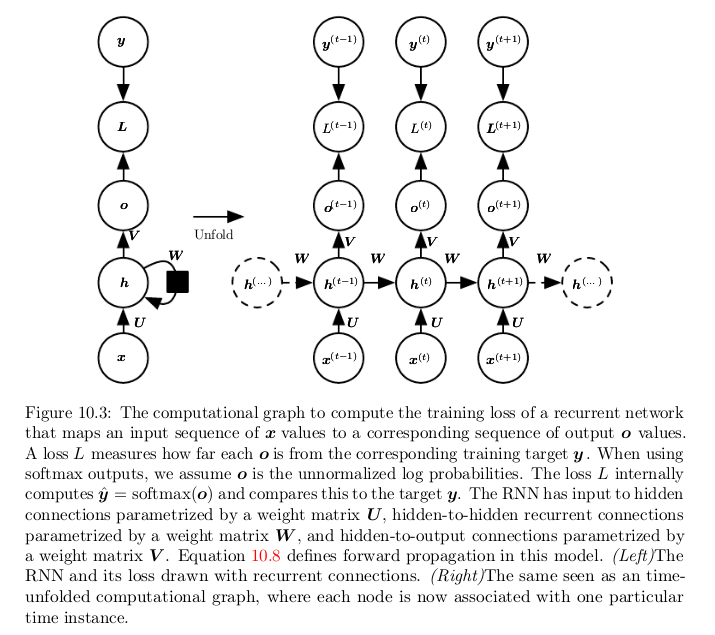
\includegraphics[width=0.7\textwidth]{rnn_dp_1.png}
\end{figure}


- RNNs that produce an output at each time step and have recurrent connections only from the output at one time step to the hidden units at the next time step 

\begin{figure}[h]
  \centering
  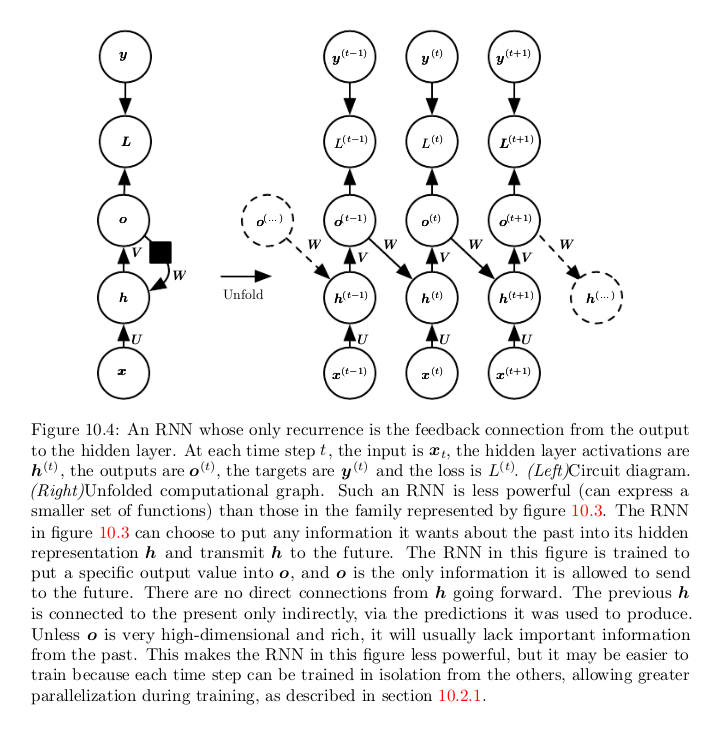
\includegraphics[width=0.7\textwidth]{rnn_dp_2.png}
\end{figure}

- RNNs with recurrent connections between hidden units that read an entire sequence and then produce a single output 

\begin{figure}[h]
  \centering
  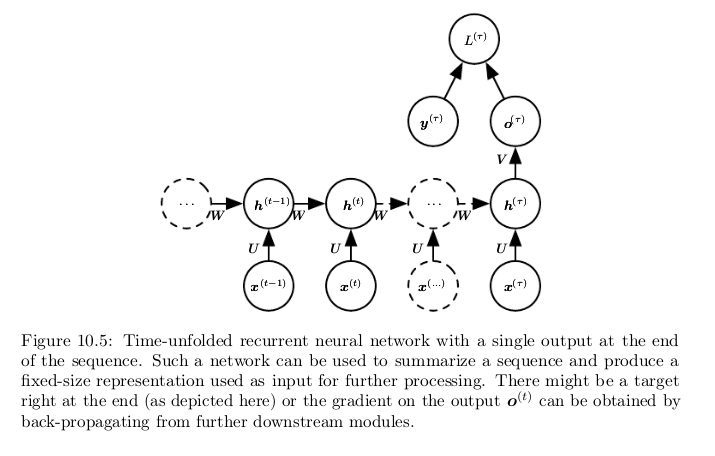
\includegraphics[width=0.7\textwidth]{rnn_dp_3.png}
\end{figure}

Any function computable by a Turing machine can be computed by a recurrent network of a finite size. The RNN, when used as a Turing machine, takes a binary sequence as input and its outputs must be discretized to provide a binary output. 

\href{https://www.sciencedirect.com/science/article/pii/089396599190080F}{Siegelmann and Sontag | Turing Computability with Neural Nets}

\begin{quote}
  \textbf{Abstract: } This paper shows the existence of a finite
  neural network, made up of sigmoidal neurons, which simulates a
  universal Turing machine. It is composed of less than 105
  synchronously evolving processors, interconnected
  linearly. High-order connections are not required.
\end{quote}

\subsection{Teacher Forcing and Networks with Output Recurrence}

The network with recurrent connections only from the output at one time step to the hidden units at the next time step is strictly less powerful because it lacks hidden to hidden recurrent connections. For example, it cannot simulate a universal Turing machine. 

The advantage of eliminating hidden to hidden recurrence is that, for any loss function based on comparing the prediction at time t to the training target at time t, all the steps are decoupled. Training can thus be parallelized with the gradient for each step t computed in isolation. 

Models that have recurrent connections from their outputs leading back into the model may be trained with \textbf{teacher forcing}. 

\begin{figure}[h]
  \centering
  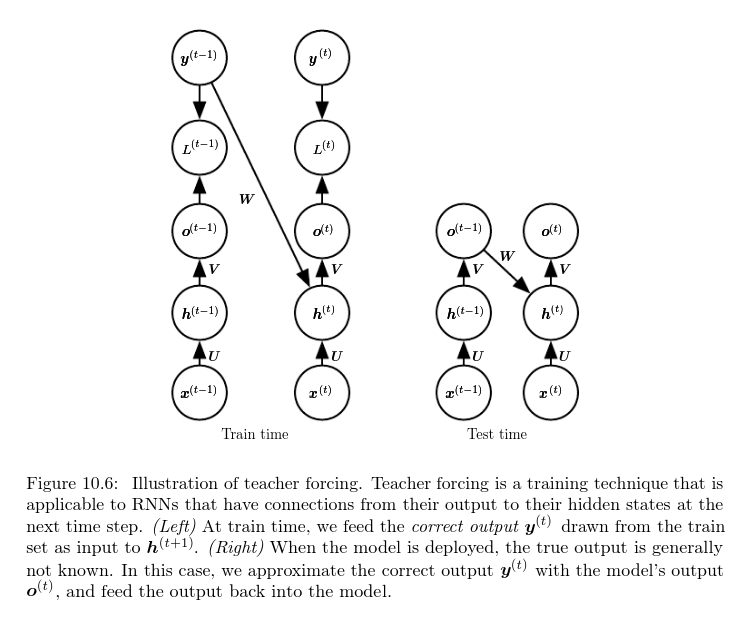
\includegraphics[width=0.7\textwidth]{teacher_forcing.png}
\end{figure}

Teacher forcing is motivated by its ability to avoid backpropagation through time in models that lack hidden to hidden connections as long as they have connections from the output at one time step to values computed in the next time step. As soon as the hidden units become a function of earlier time steps, the backpropagation through time algorithm is necessary. Some models can be trained with both teacher forcing and BPTT.

The disadvantage of strict teacher forcing arises if the network is going to be used later in a \textbf{closed loop mode}, with the network outputs fed back as input. 

An alternative mentioned is curriculum learning, which mitigates the gap between the inputs seen at training time and the inputs seen at test time randomly chooses to use generated values or actual data values as output. This approach gradually uses more of the generated values as input. 

\href{https://arxiv.org/pdf/1506.03099.pdf}{Bengio et al | Scheduled Sampling for Sequence Prediction with Recurrent Neural Networks}

\begin{quote}
  \textbf{Abstract: }

  Recurrent Neural Networks can be trained to produce sequences of
  tokens given some input, as exemplified by recent results in machine
  translation and image captioning. The current approach to training
  them consists of maximizing the likelihood of each token in the
  sequence given the current (recurrent) state and the previous
  token. At inference, the unknown previous token is then replaced by
  a token generated by the model itself. This discrepancy between
  training and inference can yield errors that can accumulate quickly
  along the generated sequence.  We propose a curriculum learning
  strategy to gently change the training process from a fully guided
  scheme using the true previous token, towards a less guided scheme
  which mostly uses the generated token instead. Experiments on
  several sequence prediction tasks show that this approach yields
  significant improvements.  Moreover, it was used successfully in our
  winning entry to the MSCOCO image captioning challenge, 2015.

\end{quote}

Extensions to teacher learning are mentioned \href{https://machinelearningmastery.com/teacher-forcing-for-recurrent-neural-networks/}{here}. 

\subsection{Computing the Gradient in a Recurrent Network}

We use the generalized backpropagation through time algorithm. BPTT begins by unfolding a recurrent network in time. The unfolded network contains k inputs and outputs, but every copy of the network shares the same parameters. Then the backpropagation algorithm is used to find the gradient of the cost with respect to all the network parameters. 

The downside to BPTT is that it has difficulty with local optima. With RNNs, local optima are a more significant problem than with feed forward neural networks. 

\subsection{Recurrent Networks as Directed Graphical Models}

When we use a predictive log likelihood training objective, we train the RNN to estimate the conditional distribution of the next sequence element $y^{(t)}$ given the past inputs. This means we maximize the log likelihood:

\begin{center}
  $\log{y^{(t)} | x^{(1)}, ..., x^{(t)}}$
\end{center}

or, if the model includes connections from the output at one time step to the next time step

\begin{center}
  $\log{y^{(t)} | x^{(1)}, ..., x^{(t)}, y^{(1)}, ..., y^{(t-1)}}$  
\end{center}

Decomposing the joint probability over the sequence of $y$ values as a series of one step probabilistic predictions is one way to capture the full joint distribution across the whole sequence. 

When we \textbf{don't} feed past $y$ values as inputs that condition the next step prediction, the directed graphical model contains no edges from any $y^{(i)}$ in the past to the current $y^{(t)}$ value. In this case, the outputs $y$ are conditionally independent given the sequence of $x$ values. 

When we do feed the actual $y$ values (the observed, actual values) back into the network, the directed graphical model contains edges from all $y^{(i)}$ values in the past to the current $y^{(t)}$ value. 

The edges in a graphical model indicate which variables depend directly on other variables. If we regard hidden units as random variables, then including them reveals that the RNN provides an efficient parameterization of the joint distribution over the observations. The price recurrent networks pay for their reduced number of parameters is that optimizing the parameters may be difficult. 

\subsection{Modeling Sequences Conditioned on Context with RNNs}

Some common ways of providing an extra input to an RNN are

\begin{enumerate}
\item as an extra input at each step
\item as the initial state $h^{(0)}$
\item both
\end{enumerate}


\begin{figure}[h]
  \centering
  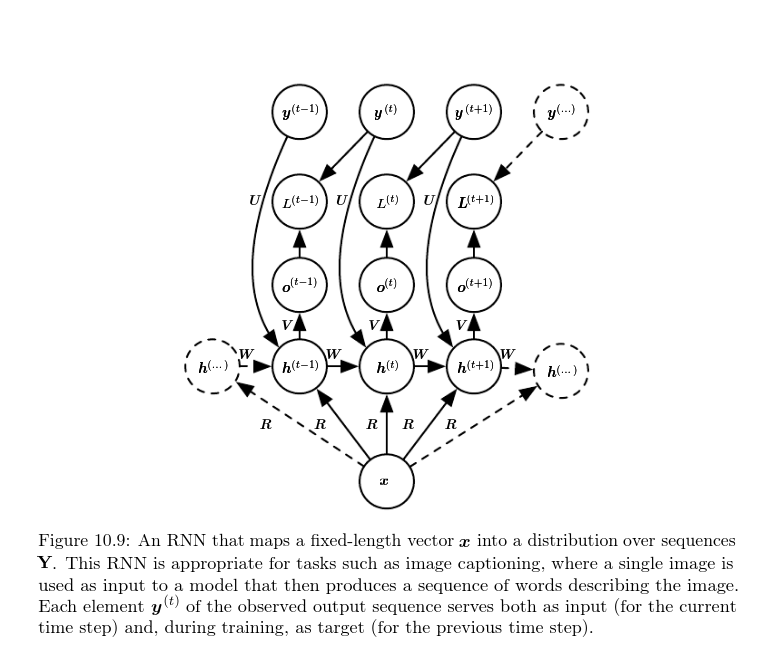
\includegraphics[width=0.7\textwidth]{context_1.png}
\end{figure}

\begin{figure}[h]
  \centering
  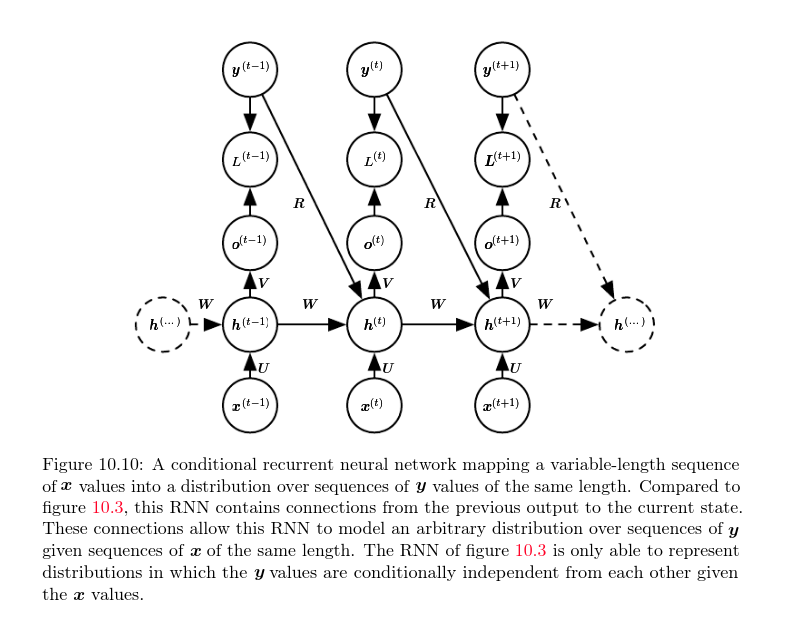
\includegraphics[width=0.7\textwidth]{context_2.png}
\end{figure}


\end{document}

